%\documentstyle[epsf,twocolumn]{jarticle}       %LaTeX2e仕様
\documentclass[twocolumn]{jarticle}     %pLaTeX2e仕様(platex.exeの場合)
% \documentclass[onecolumn]{ujarticle}   %pLaTeX2e仕様(uplatex.exeの場合)
%%%%%%%%%%%%%%%%%%%%%%%%%%%%%%%%%%%%%%%%%%%%%%%%%%%%%%%%%%%%%%
%%
%%  基本バージョン
%%
%%%%%%%%%%%%%%%%%%%%%%%%%%%%%%%%%%%%%%%%%%%%%%%%%%%%%%%%%%%%%%%%
\setlength{\topmargin}{-45pt}
%\setlength{\oddsidemargin}{0cm}
\setlength{\oddsidemargin}{-7.5mm}
%\setlength{\evensidemargin}{0cm}
\setlength{\textheight}{24.1cm}
%setlength{\textheight}{25cm}
\setlength{\textwidth}{17.4cm}
%\setlength{\textwidth}{172mm}
\setlength{\columnsep}{11mm}

%\kanjiskip=.07zw plus.5pt minus.5pt


% 【節が変わるごとに (1.1)(1.2) … (2.1)(2.2) と数式番号をつけるとき】
%\makeatletter
%\renewcommand{\theequation}{%
%\thesection.\arabic{equation}} %\@addtoreset{equation}{section}
%\makeatother

%\renewcommand{\arraystretch}{0.95} 行間の設定
%%%%%%%%%%%%%%%%%%%%%%%%%%%%%%%%%%%%%%%%%%%%%%%%%%%%%%%%
%\usepackage{graphicx}   %pLaTeX2e仕様(\documentstyle ->\documentclass)
\usepackage[dvipdfmx]{graphicx}
\usepackage{subcaption}
\usepackage{multirow}
\usepackage{amsmath}
\usepackage{url}
\usepackage{ulem}
\usepackage{algorithm}
\usepackage{algorithmic}
\usepackage{listings} %,jlisting} %日本語のコメントアウトをする場合jlistingが必要
%ここからソースコードの表示に関する設定
\lstset{
  basicstyle={\ttfamily},
  identifierstyle={\small},
  commentstyle={\smallitshape},
  keywordstyle={\small\bfseries},
  ndkeywordstyle={\small},
  stringstyle={\small\ttfamily},
  frame={tb},
  breaklines=true,
  columns=[l]{fullflexible},
  numbers=left,
  xrightmargin=0zw,
  xleftmargin=3zw,
  numberstyle={\scriptsize},
  stepnumber=1,
  numbersep=1zw,
  lineskip=-0.5ex
}
%%%%%%%%%%%%%%%%%%%%%%%%%%%%%%%%%%%%%%%%%%%%%%%%%%%%%%%%
\begin{document}

	%bibtex用の設定
	%\bibliographystyle{ujarticle}

	\twocolumn[
		\noindent
		\hspace{1em}
		2020 年 10 月 30 日
		ゼミ資料
		\hfill
		B4 杉山 竜弥
		\vspace{2mm}

		\hrule
		\begin{center}
			{\Large \bf 進捗報告}
		\end{center}
		\hrule
		\vspace{9mm}
	]

\section{今週やったこと}
\begin{itemize}
  \item いろいろなアーキテクチャの評価実験
\end{itemize}

\section{実験}

ランダムなアーキテクチャの性能,
探索を進めた時の性能と比較した.

\begin{table}[tb]
  \begin{center}
    \caption{実験の設定}
    \begin{tabular}{|c|c|} \hline
      base model & VGG19 \\ \hline
      Optim($w$) & SGD(lr=0.0090131, momentum=0.9) \\ \hline
      % Optim($\alpha$) & Adam(lr=0.005, $\beta$=(0.5, 0.999)) \\ \hline
      Scheduler($w$) & Step($\gamma$=0.2344, stepsize=100) \\ \hline
      Loss & Cross Entropy Loss \\ \hline
      dataset & cifar10 \\ \hline
      batch size & 64 \\ \hline
      epoch & 150 \\ \hline
    \end{tabular}
    \label{tab:setting}
  \end{center}
\end{table}

表\ref{tab:setting}に評価時の実験設定を示した.


\subsection{結果}

% 評価時のグラフは./graphを参照.
表\ref{tab:accg}にはテスト精度の結果を示した.
ランダムアーキテクチャは50 epochの時のショートカット数と同じにした.

\begin{table*}[t]
  \begin{center}
    \caption{各アーキテクチャの精度}
    \begin{tabular}{|c|c|c|c|c|}
    \hline
    \multicolumn{2}{|c|}{architecture} & \textbf{\begin{tabular}[c]{@{}c@{}}test accuracy\\ (\%)\end{tabular}} & \textbf{\begin{tabular}[c]{@{}c@{}}param\\ (M)\end{tabular}} & \textbf{\begin{tabular}[c]{@{}c@{}}number of\\ shortcuts\end{tabular}} \\ \hline
    \multirow{3}{*}{\begin{tabular}[c]{@{}c@{}}architecture\\ search\end{tabular}} & 50 epoch & 93.70 $\pm$ 0.22 & 21.06 $\pm$ 0.07 & 12.7 $\pm$ 1.4 \\ \cline{2-5}
     & 100 epoch & 94.02 $\pm$ 0.12 & 21.50 $\pm$ 0.11 & 18.2 $\pm$ 0.9 \\ \cline{2-5}
     & 150 epoch & 93.90 $\pm$ 0.17 & 21.57 $\pm$ 0.25 & 18.9 $\pm$ 0.6 \\ \hline
    \multicolumn{2}{|c|}{random architect} & 93.60 $\pm$ 0.15 & 21.50 $\pm$ 0.23 & 12.7 $\pm$ 1.4 \\ \hline
    \multicolumn{2}{|c|}{baseline (VGG19)} & 93.03 $\pm$ 0.10 & 20.04 & 0 \\ \hline
    \end{tabular}
    \label{tab:accg}
  \end{center}
\end{table*}

% \begin{figure}[tb]
% 	\begin{center}
% 		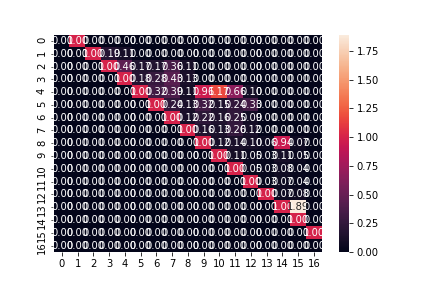
\includegraphics[clip,width=75mm]{alpha_50.png}
% 		\caption{$\alpha$ epoch 50}
% 		\label{fig:alpha50}
% 	\end{center}
% \end{figure}

\begin{figure*}[tb]
 \begin{minipage}{0.5\hsize}
 	\begin{center}
 		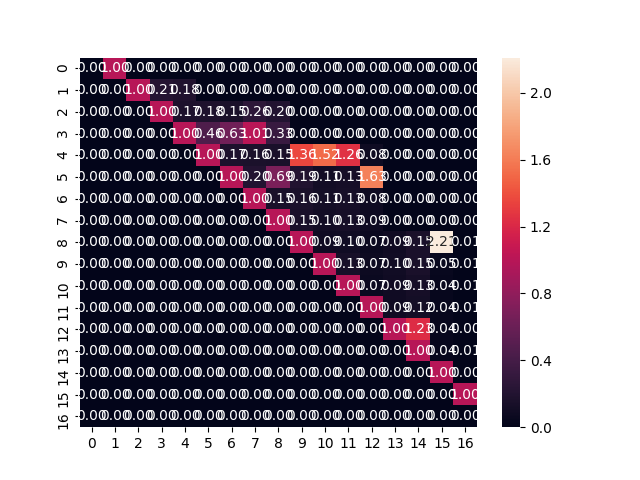
\includegraphics[clip,width=75mm]{alpha_100.png}
 		\caption{$\alpha$ epoch 100 : search}
 		\label{fig:alpha100}
 	\end{center}
 \end{minipage}
 \begin{minipage}{0.5\hsize}
 	\begin{center}
 		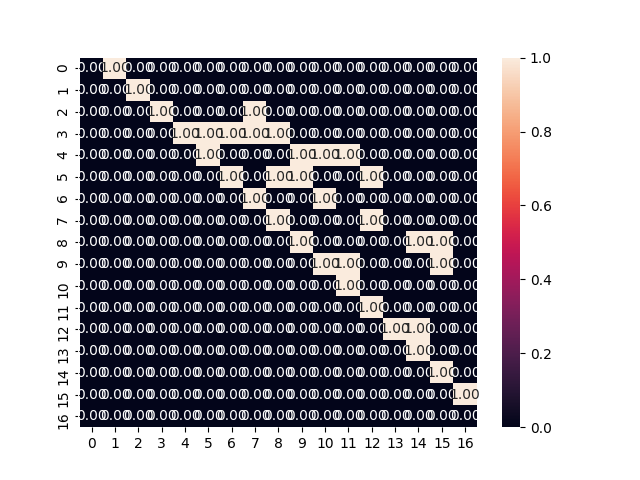
\includegraphics[clip,width=75mm]{alpha_100e.png}
 		\caption{$\alpha$ epoch 100 : eval}
 		\label{fig:alpha100e}
 	\end{center}
 \end{minipage}
\end{figure*}

\begin{figure*}[tb]
 \begin{minipage}{0.5\hsize}
 	\begin{center}
 		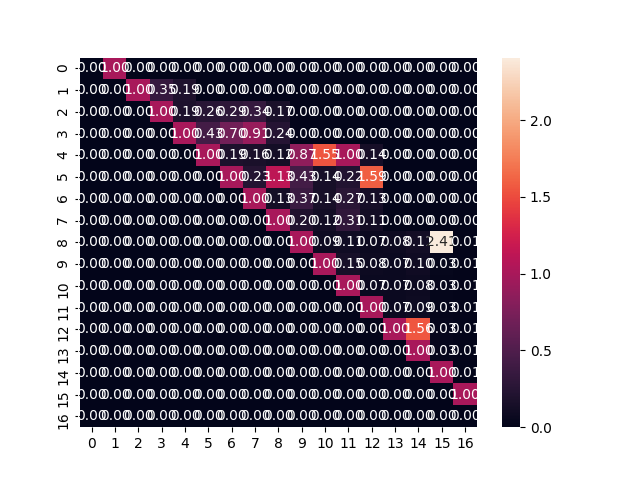
\includegraphics[clip,width=75mm]{alpha_150.png}
 		\caption{$\alpha$ epoch 150 : search}
 		\label{fig:alpha150}
 	\end{center}
 \end{minipage}
 \begin{minipage}{0.5\hsize}
 	\begin{center}
 		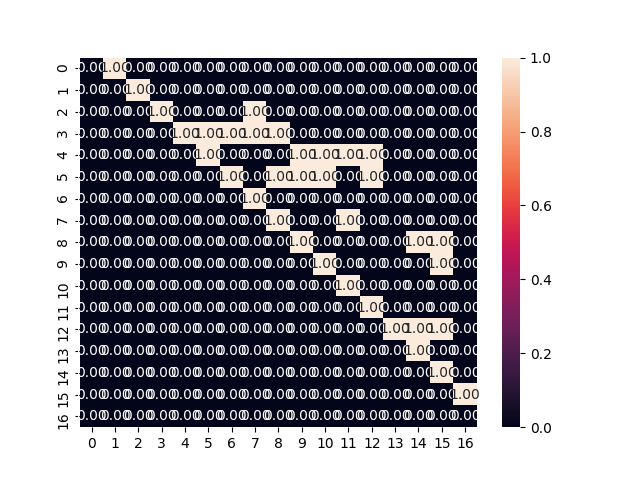
\includegraphics[clip,width=75mm]{alpha_150e.png}
 		\caption{$\alpha$ epoch 150 : eval}
 		\label{fig:alpha150e}
 	\end{center}
 \end{minipage}
\end{figure*}

\section{考察}
ランダムアーキテクチャに対して, 探索したアーキテクチャは0.1\%高い精度となった.
多少は探索の効果があると言えなくもない.

また探索を進めると, 100 epochでは精度は0.3\%高くなった.
位置の取り方が適切でないのか, 150 epochでは0.1\%下がった.
図\ref{fig:alpha150}, \ref{fig:alpha150e}のように
ダントツで重要な辺以外も大きい順に選択するので無駄な辺も選んでいると考えられる.
以前試していた閾値で辺を選ぶ方法で評価して結果を見たい.
% ショートカット数が18本に増え

\section{今後の予定}
% なんとなくなんかの勉強をするとかではなく具体的に

\begin{itemize}
  % \item 重みと編集距離の変化の調査
  % \item ランダムアーキテクチャとの比較
  % \item DARTのunrolling実験]
  \item 閾値方式での評価
  \item 論文の調査
\end{itemize}

\section{ソースコード}
% 埋め込みでもGitでもいいので参照できるように
githubのnotebookリポジトリ参照.

% 参考文献リスト
\bibliographystyle{unsrt}
\bibliography{ref}
\end{document}
